\begin{figure}[!ht]
\centering
\small
\resizebox{1.0\columnwidth}{!}{
\begin{tabular}{cccccccc}
 %%%%%%%%%%%%%%%%%%%%%%%%%%%%%% subgraph 1 %%%%%%%%%%%%%%%%%%%%%%%%%%%%%%
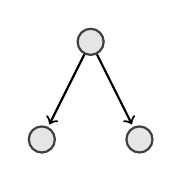
\begin{tikzpicture}[shorten >=1pt,->,scale=0.62]  
        \tikzstyle{sentence}=[circle,thick,draw=black!75,fill=black!10,minimum size=2mm]
        \tikzstyle{edge}=[draw, thick]
       \begin{scope}
         \node [sentence] (s1) at (1,2) {\tiny{}};
         \node [sentence] (s2) at (0,0) {\tiny{}};
         \node [sentence] (s3) at (2,0) {\tiny{}}; 
         \path[edge] (s1) edge [above] node[font=\tiny] {} (s2);
         \path[edge] (s1) edge [above] node[font=\tiny] {} (s3);
        \end{scope}        
      \end{tikzpicture}
&
 %%%%%%%%%%%%%%%%%%%%%%%%%%%%%% subgraph 2 %%%%%%%%%%%%%%%%%%%%%%%%%%%%%%
 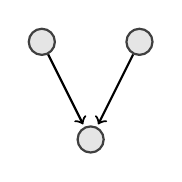
\begin{tikzpicture}[shorten >=1pt,->,scale=0.62]  
        \tikzstyle{sentence}=[circle,thick,draw=black!75,fill=black!10,minimum size=2mm]
        \tikzstyle{edge}=[draw, thick]
       \begin{scope}
         \node [sentence] (s1) at (0,2) {\tiny{}};
         \node [sentence] (s2) at (2,2) {\tiny{}};
         \node [sentence] (s3) at (1,0) {\tiny{}}; 
         \path[edge] (s1) edge [above] node[font=\tiny] {} (s3);
         \path[edge] (s2) edge [above] node[font=\tiny] {} (s3);
        \end{scope}        
      \end{tikzpicture}

&
 %%%%%%%%%%%%%%%%%%%%%%%%%%%%%% subgraph 3 %%%%%%%%%%%%%%%%%%%%%%%%%%%%%%
 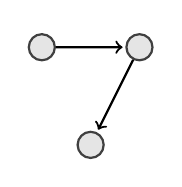
\begin{tikzpicture}[shorten >=1pt,->,scale=0.62]  
        \tikzstyle{sentence}=[circle,thick,draw=black!75,fill=black!10,minimum size=2mm]
        \tikzstyle{edge}=[draw, thick]
       \begin{scope}
         \node [sentence] (s1) at (0,2) {\tiny{}};
         \node [sentence] (s2) at (2,2) {\tiny{}};
         \node [sentence] (s3) at (1,0) {\tiny{}}; 
         \path[edge] (s1) edge [above] node[font=\tiny] {} (s2);
         \path[edge] (s2) edge [above] node[font=\tiny] {} (s3);
        \end{scope}        
      \end{tikzpicture}
      
&
 %%%%%%%%%%%%%%%%%%%%%%%%%%%%%% subgraph 4 %%%%%%%%%%%%%%%%%%%%%%%%%%%%%%
 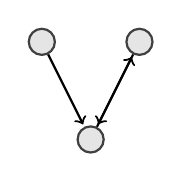
\begin{tikzpicture}[shorten >=1pt,->,scale=0.62]  
        \tikzstyle{sentence}=[circle,thick,draw=black!75,fill=black!10,minimum size=2mm]
        \tikzstyle{edge}=[draw, thick]
       \begin{scope}
         \node [sentence] (s1) at (0,2) {\tiny{}};
         \node [sentence] (s2) at (2,2) {\tiny{}};
         \node [sentence] (s3) at (1,0) {\tiny{}}; 
         \path[edge] (s1) edge [above] node[font=\tiny] {} (s3);
         \path[edge] (s2) edge [above] node[font=\tiny] {} (s3);
         \path[edge] (s3) edge [above] node[font=\tiny] {} (s2);
         
        \end{scope}        
      \end{tikzpicture}      
      
&
 %%%%%%%%%%%%%%%%%%%%%%%%%%%%%% subgraph 5 %%%%%%%%%%%%%%%%%%%%%%%%%%%%%%
 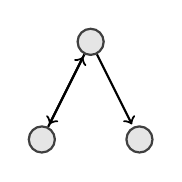
\begin{tikzpicture}[shorten >=1pt,->,scale=0.62]  
        \tikzstyle{sentence}=[circle,thick,draw=black!75,fill=black!10,minimum size=2mm]
        \tikzstyle{edge}=[draw, thick]
       \begin{scope}
         \node [sentence] (s1) at (1,2) {\tiny{}};
         \node [sentence] (s2) at (0,0) {\tiny{}};
         \node [sentence] (s3) at (2,0) {\tiny{}}; 
         \path[edge] (s2) edge [above] node[font=\tiny] {} (s1);
         \path[edge] (s1) edge [above] node[font=\tiny] {} (s2);
         \path[edge] (s1) edge [above] node[font=\tiny] {} (s3);
         
        \end{scope}        
      \end{tikzpicture}            
      
 &
 %%%%%%%%%%%%%%%%%%%%%%%%%%%%%% subgraph 6 %%%%%%%%%%%%%%%%%%%%%%%%%%%%%%
 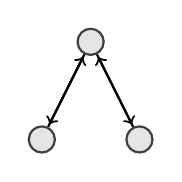
\begin{tikzpicture}[shorten >=1pt,->,scale=0.62]  
        \tikzstyle{sentence}=[circle,thick,draw=black!75,fill=black!10,minimum size=2mm]
        \tikzstyle{edge}=[draw, thick]
       \begin{scope}
         \node [sentence] (s1) at (1,2) {\tiny{}};
         \node [sentence] (s2) at (0,0) {\tiny{}};
         \node [sentence] (s3) at (2,0) {\tiny{}}; 
         \path[edge] (s2) edge [above] node[font=\tiny] {} (s1);
         \path[edge] (s1) edge [above] node[font=\tiny] {} (s2);
         \path[edge] (s1) edge [above] node[font=\tiny] {} (s3);
         \path[edge] (s3) edge [above] node[font=\tiny] {} (s1);
         
        \end{scope}        
      \end{tikzpicture}            
      
 &
 %%%%%%%%%%%%%%%%%%%%%%%%%%%%%% subgraph 7 %%%%%%%%%%%%%%%%%%%%%%%%%%%%%%
 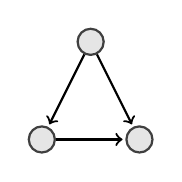
\begin{tikzpicture}[shorten >=1pt,->,scale=0.62]  
        \tikzstyle{sentence}=[circle,thick,draw=black!75,fill=black!10,minimum size=2mm]
        \tikzstyle{edge}=[draw, thick]
       \begin{scope}
         \node [sentence] (s1) at (1,2) {\tiny{}};
         \node [sentence] (s2) at (0,0) {\tiny{}};
         \node [sentence] (s3) at (2,0) {\tiny{}}; 
         
         \path[edge] (s1) edge [above] node[font=\tiny] {} (s2);
         \path[edge] (s1) edge [above] node[font=\tiny] {} (s3);
         \path[edge] (s2) edge [above] node[font=\tiny] {} (s3);
         
        \end{scope}        
      \end{tikzpicture}            
      
 &
 %%%%%%%%%%%%%%%%%%%%%%%%%%%%%% subgraph 8 %%%%%%%%%%%%%%%%%%%%%%%%%%%%%%
 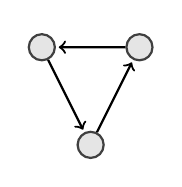
\begin{tikzpicture}[shorten >=1pt,->,scale=0.62]  
        \tikzstyle{sentence}=[circle,thick,draw=black!75,fill=black!10,minimum size=2mm]
        \tikzstyle{edge}=[draw, thick]
       \begin{scope}
         \node [sentence] (s1) at (0,2) {\tiny{}};
         \node [sentence] (s2) at (2,2) {\tiny{}};
         \node [sentence] (s3) at (1,0) {\tiny{}}; 
         
         \path[edge] (s2) edge [above] node[font=\tiny] {} (s1);
         \path[edge] (s1) edge [above] node[font=\tiny] {} (s3);
         \path[edge] (s3) edge [above] node[font=\tiny] {} (s2);
         
        \end{scope}        
      \end{tikzpicture}  
\\

&
 %%%%%%%%%%%%%%%%%%%%%%%%%%%%%% subgraph 9 %%%%%%%%%%%%%%%%%%%%%%%%%%%%%%
 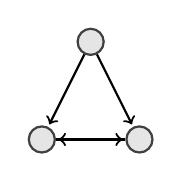
\begin{tikzpicture}[shorten >=1pt,->,scale=0.62]  
        \tikzstyle{sentence}=[circle,thick,draw=black!75,fill=black!10,minimum size=2mm]
        \tikzstyle{edge}=[draw, thick]
       \begin{scope}
         \node [sentence] (s1) at (1,2) {\tiny{}};
         \node [sentence] (s2) at (0,0) {\tiny{}};
         \node [sentence] (s3) at (2,0) {\tiny{}}; 
         
         \path[edge] (s1) edge [above] node[font=\tiny] {} (s2);
         \path[edge] (s1) edge [above] node[font=\tiny] {} (s3);
         \path[edge] (s3) edge [above] node[font=\tiny] {} (s2);
         \path[edge] (s2) edge [above] node[font=\tiny] {} (s3);
         
        \end{scope}        
      \end{tikzpicture}             
&
%%%%%%%%%%%%%%%%%%%%%%%%%%%%%% subgraph 10 %%%%%%%%%%%%%%%%%%%%%%%%%%%%%%
 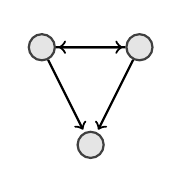
\begin{tikzpicture}[shorten >=1pt,->,scale=0.62]  
        \tikzstyle{sentence}=[circle,thick,draw=black!75,fill=black!10,minimum size=2mm]
        \tikzstyle{edge}=[draw, thick]
       \begin{scope}
         \node [sentence] (s1) at (0,2) {\tiny{}};
         \node [sentence] (s2) at (2,2) {\tiny{}};
         \node [sentence] (s3) at (1,0) {\tiny{}}; 
         
         \path[edge] (s1) edge [above] node[font=\tiny] {} (s2);
         \path[edge] (s2) edge [above] node[font=\tiny] {} (s1);
         \path[edge] (s1) edge [above] node[font=\tiny] {} (s3);
         \path[edge] (s2) edge [above] node[font=\tiny] {} (s3);
         
        \end{scope}        
      \end{tikzpicture}  

 &
 %%%%%%%%%%%%%%%%%%%%%%%%%%%%%% subgraph 11 %%%%%%%%%%%%%%%%%%%%%%%%%%%%%%
 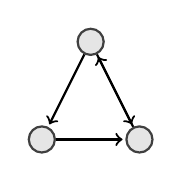
\begin{tikzpicture}[shorten >=1pt,->,scale=0.62]  
        \tikzstyle{sentence}=[circle,thick,draw=black!75,fill=black!10,minimum size=2mm]
        \tikzstyle{edge}=[draw, thick]
       \begin{scope}
         \node [sentence] (s1) at (1,2) {\tiny{}};
         \node [sentence] (s2) at (0,0) {\tiny{}};
         \node [sentence] (s3) at (2,0) {\tiny{}}; 
         
         \path[edge] (s1) edge [above] node[font=\tiny] {} (s2);
         \path[edge] (s1) edge [above] node[font=\tiny] {} (s3);
         \path[edge] (s3) edge [above] node[font=\tiny] {} (s1);
         \path[edge] (s2) edge [above] node[font=\tiny] {} (s3);
         
        \end{scope}        
      \end{tikzpicture}             

&
%%%%%%%%%%%%%%%%%%%%%%%%%%%%%% subgraph 12 %%%%%%%%%%%%%%%%%%%%%%%%%%%%%%
 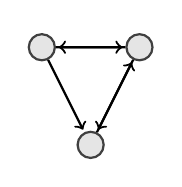
\begin{tikzpicture}[shorten >=1pt,->,scale=0.62]  
        \tikzstyle{sentence}=[circle,thick,draw=black!75,fill=black!10,minimum size=2mm]
        \tikzstyle{edge}=[draw, thick]
       \begin{scope}
         \node [sentence] (s1) at (0,2) {\tiny{}};
         \node [sentence] (s2) at (2,2) {\tiny{}};
         \node [sentence] (s3) at (1,0) {\tiny{}}; 
         
         \path[edge] (s1) edge [above] node[font=\tiny] {} (s2);
         \path[edge] (s2) edge [above] node[font=\tiny] {} (s1);
         \path[edge] (s1) edge [above] node[font=\tiny] {} (s3);
         \path[edge] (s2) edge [above] node[font=\tiny] {} (s3);
         \path[edge] (s3) edge [above] node[font=\tiny] {} (s2);
         
        \end{scope}        
      \end{tikzpicture}  
&
%%%%%%%%%%%%%%%%%%%%%%%%%%%%%% subgraph 13 %%%%%%%%%%%%%%%%%%%%%%%%%%%%%%
 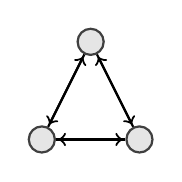
\begin{tikzpicture}[shorten >=1pt,->,scale=0.62]  
        \tikzstyle{sentence}=[circle,thick,draw=black!75,fill=black!10,minimum size=2mm]
        \tikzstyle{edge}=[draw, thick]
       \begin{scope}
         \node [sentence] (s1) at (1,2) {\tiny{}};
         \node [sentence] (s2) at (0,0) {\tiny{}};
         \node [sentence] (s3) at (2,0) {\tiny{}}; 
         
         \path[edge] (s1) edge [above] node[font=\tiny] {} (s2);
         \path[edge] (s2) edge [above] node[font=\tiny] {} (s1);

         \path[edge] (s2) edge [above] node[font=\tiny] {} (s3);
         \path[edge] (s3) edge [above] node[font=\tiny] {} (s2);
         
         \path[edge] (s1) edge [above] node[font=\tiny] {} (s3);
         \path[edge] (s3) edge [above] node[font=\tiny] {} (s1);
         
        \end{scope}        
      \end{tikzpicture} 
      &
      
\end{tabular}
}
\caption{All possible directed 3\-- node subgraphs.}
\label{f:all_3node_subgraphs}
\end{figure}